\documentclass[pdf,titlepage,a4paper]{report}

\usepackage{graphicx}
\usepackage{color}

\usepackage{fancyhdr}
\setlength{\headheight}{24pt}
\pagestyle{fancy}
\rhead{
\includegraphics[scale=0.2]{Graphics/nav-logo.png}}
\chead{فاز یک پروژه پیشرفته}

\usepackage[hidelinks]{hyperref}

\usepackage[fontsize=18pt]{fontsize}


%\usepackage[top=2cm, bottom=2cm, outer=0cm, inner=0cm]{geometry}
\usepackage{background}

\backgroundsetup{
	scale=1,
	color=white,
	opacity=0.4,
	angle=0,
	contents={%
		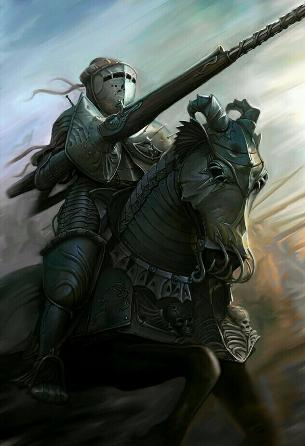
\includegraphics[width=\paperwidth,height=\paperheight]{Graphics/0d430388ec86043008f3ddd51b87958a.jpeg}
	}%
}

\usepackage{indentfirst}
\usepackage{xepersian}
\settextfont{B Zar}

%\newcommand{\s}{\fontdimen2\font=0.125em}

\begin{titlepage}
	\title{
\includegraphics[scale=0.8]{Graphics/BASU_logo.png} \\ \Huge{فاز یک پروژه پیشرفته}}
	\author{متین امیرپناه فر \\ شماره داشنجویی : 40212358003
		  \and \\ نیما مخملی \\ شماره داشنجویی : 40212358035}
	\date{\today}
\end{titlepage}

\renewcommand{\labelitemi}{$\bullet$}

\begin{document}
	{\color{white}
	\maketitle}
	\tableofcontents
	\newpage

	\begin{abstract}
		
		در دورانی که قلمرو شاهی به استان های خود مختار تقسیم شده،سردارانی از گوشه ی سرزمین در سودای کشورگشایی،ارتش خود را برای فتح شهرها گسیل داشته اند.تا با مهارت و شجاعت بجنگند و با تدبیر و مکر به حریفان رکب بزنند تا قدرت و افتخار کسب کنند \\

     بازی رکب یک بازی تخته ای است که توسط 3 تا 6 بازیکن انجام میشود 
	 این بازی شامل دو نوع کارت بنفش و زرد است که هر کارت بنفش امتیاز خاص خود را دارد ولی کارت های زرد ویژگی خاصی ندارند
	 کارت های بنفش عبارتند از : مترسک , طبل زن , شاهدخت ,  شیرزن  ,  بهار  , زمستان , ریش سفید 
	 بازیکنان باید با کارت هایی که در دست دارند به جنگ بپردازند و سعی کنند در جنگ پیروز شوند و اگر سه استان مجاور یا پنج استان را فتح کنند پیروز کل بازی خواهند شد 
	 ما این بازی را به صورت شی گرا نوشته ایم که شرح کلاس ها و قابلیت های آنها را در ادامه برایتان میگوییم
	  
	\end{abstract}
    
	\newpage
    \part{نحوه بازی}
     هنگامی که بازی را آغاز مینماییم در ورودی از کاربر میخواهد که تعداد بازیکنان را وارد کند. \\
     \indent سپس هر بازیکن مشخصات خود را وارد میکند و بعد رنگ نشان خود را انتخاب میکنند.
	 بعد از آن سیستم چک میکند و کم سن ترین بازیکن را به عنوان اولین بازی کن که جنگ اول را شروع میکند برمیگزیند.\\
	 \indent بازیکن موردنظر استان محل اولین جنگ را انتخاب میکند و سپس سیستم کارت های بازیکنان را به صورت رندوم به آنها میدهد. \\
	 در خروجی برنامه از بازیکنان میخواهد که به صورت خصوصی کارت های خود را مشاهده کنند و به ترتیب این عمل انجام میشود\\
	 آنگاه بازی توسط بازیکن کم سن آغاز میشود و به ترتیب سن بازیکن ها کارت های خود را رو میکنند\\
	 بازیکنان میتوانند کارت هارا رو کنند تا بالاخره فاتح استان مورد جنگ معلوم شود\\
	 و به همین ترتیب بازی را ادامه میدهند تا یک بازیکن 3 استان مجاور یا 5 استان از کل نقشه را فتح کند.\\
	
	\part{کلاس ها}
		
	\newpage
	\section{بازی}
	این کلاس وظیفه اصلی و مدیریت کلی بازی را بر عهده دارد شرایط بازی را آماده و بازیکنان را مجهز و آماده جنگ میکند
	این کلاس با کلاس های بازیکن , زمین بازی , رابط کاربری , تمام کلاس های کارت ها و تمام کلاس های نشان رابطه دارد
	\paragraph{روابط}
	این کلاس با کلاس های بازیکن , زمین بازی , تمام کارت ها ,تمام نشان ها و رابط کاربری رابطه دارد.\\
	رابط بین این کلاس ها همه از نوع \Ir{composition}میباشد.\\
	\paragraph{صفات}
	صفات این بازی عبارتند از آرایه ای از تمام کارت های بازی مانند آرایه هایی از کارت های بنفش با تعداد مختلف
	همچنین اشیاء مورد نیاز این کلاس از کلاس هایی مانند
	\begin{latin}
		\begin{itemize}
			\item \lr{ui}
			\item \lr{gameboard}
			\item \lr{battlemarker}
			\item \lr{player}
		\end{itemize}
	\end{latin}
	\paragraph{متدها}
	\begin{latin}
		\begin{itemize}
			\item \lr{play} این تابع وظایف شروع و مدیریت بازی را دارد
			\item \lr{gethelp} برای ارسال متن راهنمایی است
			\item \lr{check\_number\_of\_player} چک کردن 
			\item \lr{set\_battleground} ست کردن محل جنگ
			\item \Ir{find\_war\_winner} پیدا کردن برنده جنگ 
			\item \Ir{find\_game\_winner} پیدا کردن برنده کل بازی 
			\item \Ir{getPlayers} ارسال بازیکنان البته اطلاعات بازیکنان
			\item \Ir{shuffle} مخلوط کردن کارت ها
			\item \Ir{distributeCards} پخش کارت ها
			\item \Ir{war} این تابع برای مدیریت جنگ است
		\end{itemize}
	\end{latin}
	\newpage
	\section{رابط کاربری}
	این کلاس وظیفه برقراری ارتباط سیستم و کاربران را دارد دستورات را از ورودی میگیرد و گزارشات را در خروجی برای رویت کردن کاربران چاپ میکند\\
    ین کلاس صفتی که به شکل خصوصی باشد ندارد 
	\paragraph{روابط}
	
	\paragraph{متدها}
	متد ها یا رفتار های این کلاس عبارتند از 
	\begin{latin}
		\begin{itemize}
			\item \Ir{clearTerminal}  پاک کردن تصویر 
			\item \Ir{pause}  توقف چند لحظه ای 
			\item \Ir{spliter}  خوشگلاسیون
			\item \Ir{showPlayerPlayedCards} نمایش کارت های بازی شده بازیکنان
			\item \Ir{getCommand} برای انتخاب ویژگی های خاص بازی من جمله پاس دادن
			\item \Ir{get\_battleground} مکان جنگ
			\item \Ir{showPlayerStates}  نمایش استان های فتح شده بازیکن 
			\item \Ir{showPlayerCards}  نمایش کارت های در دست بازیکن
			\item \Ir{get\_card\_name} ارسال نام کارت ها
			\item \It{get\_players\_number}  ارسال شماره بازیکن البته به ترتیب سن
			\item \Ir{get\_player\_name}  ارسال نام بازیکن
			\item \Ir{get\_player\_old}   ارسال نام بازیکن
			\item \Ir{get\_player\_color}  ارسال رنگ بازیکن 
			\item \Ir{declare\_warWinner} برنده جنگ
			\item \Ir{declare\_gameWinner}  برنده کل بازی 
		\end{itemize}
	\end{latin}
	
	\newpage
	\section{رابط گرافیکی}
	 این کلاس در فاز های بعدی پروژه اضافه خواهد شد. \\
	 که قرار است این کار را با محیط توسعه کیو تی انجام دهیم.
	\paragraph{صفات}
	\paragraph{متدها}


	\newpage
	\section{زمین بازی}
    این کلاس ارتباط بین استان هارا معلوم کرده و در واقع همان صفحه کاغذی موجود در بازی است \\
    این کلاس برای ما استان های بازی را نگهداری کرده و ارتباط بین آنها را ایجاد میکند و مشخص میکند که آیا دو استان با هم مجاورند یا خیر 
    \paragraph{روابط}
	این کلاس با کلاس ایالت رابطه دارد که این رابطه نوعی رابطه وابستگی را بین آنها شرح میدهد.\\
	\paragraph{صفات}
	صفات خصوصی این کلاس استان های بازی هستند که شامل 14 استان میشوند 
	این استان ها با استفاده از \lr{unordered\_map} و کلاس استان گرفته شده اند
	و صفت بعدی ارتباط بین این استان هاست که برای این کار از کلاس \lr{map} استفاده کرده ایم
	\paragraph{متدها}
	
	متد های این کلاس عبارتند از :

		\begin{itemize}
			\item \lr{checkAdjacency} برای چک کردن 
			\item \lr{getState} ارسال استان های بازی 
			\item \lr{get\_active\_states\_name} ارسال نام استان فعال و منتخب
		\end{itemize}
	
	\newpage
	\section{کارت ها}
	این کلاس مسئول نگهداری و سازماندهی کارت هاست این کلاس دو زیر کلاس دارد که بیانگر دو نوع کارت بنفش و زرد ایست که در بازی داریم
    \paragraph{روابط}
    این کلاس با کلاس های بازی و بازیکن رابطه دارد
	این روابط از نوع \Ir{assosiation} و \Ir{compositon} است.\\
	\paragraph{صفات}
	صفات کلاس کارت ها  عبارتند از 
	\begin{enumerate}
		\item امتیاز که این کلاس چون دو کلاس از آن ارث بری میکنند صفت امتیاز را به صورت \lr{protected}  نوشته ایم
		\item  ویژگی اولویت که به صورت خصوصی است
	\end{enumerate}

	\paragraph{متدها}
	توابع که برای این کلاس تعریف کرده ایم :

	\begin{itemize}
		\item \lr{getType} ارسال نوع کارت مدنظر
		\item \lr{applyFeature} ویژگی کارت های ویژه یا بنفش که برای هر کارت به صورت جداگانه تعریف شده است
		\item \lr{is\_season} چک کردن اینکه آیا کارت فصل است یا خیر؟
		\item \lr{getPriority} ارسال اولویت کارت برای امور بازی 
		\item \lr{setPoint}  قرار دادن امتیاز
		\item \lr{getPoint} ارسال امتیاز مربوط به کارت
	\end{itemize}
	
	
	\subsection{کارت های بنفش(ویژه)}
	این کلاس برای کارت های ویژه این بازی طراحی شده است که تمام کلاس های شخصیت های کلاس بنفش از این کلاس ارث بری میکنند
	کلاس هایی همچون 
	\begin{itemize}
		\item \lr{bishop}
		\item \lr{drummer}
		\item \lr{heroine}
		\item \lr{scarecrow}
		\item \lr{spring}
		\item \lr{spy}
		\item \lr{turncoat}
		\item \lr{winter}  
	\end{itemize}
	\paragraph{صفات}
	این کلاس فقط یک صفت دارد که آن هم برای \lr{type}  کارتهاست
	\paragraph{روابط}
	تک تک کارت های بنفش یا شخصیت ها با کلاس کارت بنفش رابطه ارث بری دارند \\
	به همین جهت در شرح تک تک کلاس های ویژه دیگر بند روابط را نداریم.\\
	همچنین خود کلاس کارت های بنفش هم با کلاس کارت رابطه ارث بری دارد.\\

	\subparagraph{}
	
	\paragraph{متدها}
	همچنین این کلاس فقط یک تابع برای ارسال \lr{type} دارد که اسم آن \lr{getType} است
	\subsubsection{مترسک}
	کلاس شخصیت مترسک : این کارت وقتی در بازی به کار برده میشود بازیکن میتواند یک کارت زرد را به بازی برگرداند 
	این کارت روی کارت های بنفش تاثیری ندارد
	\paragraph{صفات}
	 تنها  صفت این کلاس صفت \lr{help}  است که موقعی به کار برده میشود که کاربر بخواهد توضیحات مربوط به کارت را ببیند و با کارت آشنا شود
	 
	 \paragraph{متدها}
	 توابع این کلاس عبارتند از  
	 \lr{gethelp} که برای ارسال متن توضیحات است 
	 و \lr{applyFeature} که مربوط به ویژگی کارت است
	\subsubsection{طبل زن}
	 کلاس شخصیت طبل زن : این کارت وقتی توسط یک بازیکن رو میشود ارزش تمام کارت های زردی که آن بازیکن در یک درست آورده دو برابر میشود. البته فقط یکبار امکان پذیر است.

    \paragraph{صفات}
	تنها  صفت این کلاس صفت \lr{help}  است که موقعی به کار برده میشود که کاربر بخواهد توضیحات مربوط به کارت را ببیند و با کارت آشنا شود
	\paragraph{متدها}
	توابع این کلاس عبارتند از  
	\lr{gethelp} که برای ارسال متن توضیحات است 
	و \lr{applyFeature} که مربوط به ویژگی کارت است
	\subsubsection{شاهدخت}
	 کلاس شخصیت شاهدخت : کارت شاهدخت یک کارت امتیازیه که هیچ کارت دیگری روی آن اثر ندارد.
	\paragraph{صفات}
	این کلاس فقط یک صفت دارد به نام \lr{help}  که برای نمایش توضیحات این کارت است
	\paragraph{متدها}

	 دو متد این کلاس عبارت است از : \\
	
	\begin{itemize}
		\item \lr{gethelp}  برای ارسال متن توضیحات کارت است که کاربر درخواست کمک کرده است.
		\item \lr{applyFeature} این تابع نیز برای اعمال ویژگی کارت است
	\end{itemize}
	

	\subsection{فصل ها}
    این کلاس برای فصل های بهار و زمستان که دو کارت ویژه هستند طراحی شده است که همان طور که معلوم است دو کلاس بهار و زمستان از آن ارث بری میکنند

	\paragraph{صفات}
	این کلاس هیچ عضو داده ای خصوصی ندارد.
	\paragraph{متدها}
	تنها تابع عضو داده ای این کلاس تابع \lr{is\_season} است \\ 
	که این تابع نیز برای چک کردن فصل بودن است که قبلا توضیح دادیم
	
	\subsubsection{بهار}
	 کلاس شخصیت بهار : تا زمانی که بهار باشد به مجموع کارت های رو شده بازیکن یا بازیکنانی که بالا ترین کارت عددی را رو کرده اند یا  در آینده بازی میکنن را3 واحد اضافه میکند.

	\paragraph{صفات}
	این کلاس هم مانند تمام کلاس های کارت بنفش فقط یک صفت \lr{help} دارد
	\paragraph{متدها}
	\lr{gethelp} , \lr{applyFeature} \\
	توضیحات این توابع را در کلاس های قبلی گفته ایم.

	\subsubsection{زمستان}
	کارت شخصیت زمستان : تا زمانی که زمستان باشد عدد تمام کارت های زرد یا سرباز همه بازیکنان 1 میشود اگر بهار باشد و زمستان بیاید , زمستان میشود
	\paragraph{صفات}
	\lr{help}
	\paragraph{متدها}
	\lr{gethelp} , \lr{applyFeature} \\
	مانند دیگر کلاس های کارت های ویژه

	\subsection{کارت های زرد(سرباز)}
	کارت های زرد یا سرباز موقعی که رو میشوند قدرت ارتش بازیکن را به اندازه عدد روی کارت افزایش میدهد.

	\paragraph{صفات}
	هیچ صفتی ندارد 
	\paragraph{متدها}
	این کلاس هم دو تابع \lr{gethelp} , \lr{applyFeature} را دارا میباشد
	\newpage
	
	\section{نشان}
	کلاس نشان یک کلاس پدر است که سه کلاس فرزند دارد این کلاس را از آن جهت طراحی کرده ایم که نشان های بازیکن و جنگ و صلح را پیاده سازی کنیم
	\paragraph{صفات}
     صفات این کلاس :
	 1- یک شی از کلاس \lr{State}  برای اعمال نشان جنگ
	 2- یک شی از کلاس \lr{Color} برای پیاده سازی نشان بازیکنان با رنگ های متفاوت
	\paragraph{متدها}
	 توابع عضو این کلاس :

	\begin{itemize}
		\item \lr{setState} قرار دادن استان مدنظر
		\item \lr{getState} ارسال استان مدنظر 
		\item \lr{is\_set}برای چک کردن که آیا استان منتخب است؟
	\end{itemize}
	 
	\subsection{نشان بازیکن}
	این کلاس را برای نشان بازیکن طراحی کرده ایم تا بازیکنان به هنگام آغاز بازی یک نشان برای خود انتخاب کنند و وقتی یک استان را فتح کردند آن نشان روی استان مورد نظر قرار گیرد
	\paragraph{روابط}
	 این کلاس با کلاس نشان رابطه ارث بری دارد 
	\paragraph{روابط}
	این کلاس با کلاس رنگ رابطه دارد برای ست کردن رنگ نشان هر بازیکن.\\ 
	\paragraph{صفات}
	ندارد
	\paragraph{متدها}
	ندارد
	
	\subsection{ایالت}
	کلاس ایالت یا استان به این منظور طراحی شده که فرایندی که لازم است مستقیم با استان ها انجام شود راحت تر صورت بگیرند 

	\paragraph{صفات}
	 برای این کلاس دو صفت در نظر گرفته شده است
	 \begin{latin}
	 	\begin{itemize}
	 		\item \lr{name} نام استان 
	 		\item \lr{set\_marker} قرار دادن نشان فاتح استان
	 	\end{itemize}
	 \end{latin}
	\paragraph{متدها}
	
	\section{بازیکن}
	این کلاس به منظور مدیریت بازیکنان و تمام رفتار ها و ویژگی های آنها طراحی شده است 
	 این کلاس با کلاس های کارت استان و نشان بازیکن و رابط کاربری رابطه دارد
	\paragraph{صفات}
	ویژگی های خصوصی کلاس بازیکنان شامل نام , سن , آی دی , وکتوری از کارت های در اختیار ,وکتوری از کارت های بازی شده , استان های فتح شده و آرایه ای از نشان بازیکنان.
	\paragraph{روابط}
	کلاس بازیکن با کلاس های کارت , استان , و نشان و نشان بازیکن رایطه دارد.\\
	
	\paragraph{متدها}
	توابع عضو این کلاس شامل توابع زیر میشوند :
	
	\begin{itemize}
		\item \lr{getName} برای ارسال نام بازیکنان
		\item \lr{getID} برای ارسال شماره بازیکنان
		\item \lr{getAge}  برای ارسال سن بازیکنان
		\item \lr{getPlayedCards} برای ارسال کارت های بازی شده بازیکن
		\item \lr{getCards} برای ارسال کارت های در دست بازیکنان
		\item \lr{setCards} قرار دادن کارت ها
		\item \lr{setState} قرار دادن استان مدنظر
		\item \lr{get\_states\_name} ارسال نام استان
		\item \lr{drawn\_card} کشیدن کارت برای بازی 
		\item \lr{push\_to\_cards} افزودن کارت به کارت های در دست بازیکن
		\item \lr{push\_to\_playedCards} افزودن به کارت های مصرف شده بازیکن
		\item \lr{drawn\_playedCard} کشیدن کارت های بازی شده
	\end{itemize}
	
	\newpage
	
	
	
	\part{چالش ها}
	
	چالش هایی که در برنامه نویسی این بازی با آنها مواجه شدیم عبارتند از 
	\begin{enumerate}
		\item	پیاده سازی مجاورت بودن استان های بازی که از کلاس \lr{map}  استفاده کردیم 
		\item پیاده سازی ماهیت استان ها با استفاده از \lr{unordered\_map} 
		\item کامپایل کردن و اجرای برنامه توسط \lr{CMAKE} (اجرای برنامه ای با چندین فایل)
    	\item برقراری ارتباط بین کلاس ها  ایجاد بستری برای اجرای برنامه توسط رابط گرافیکی \lr{QT}
	    \item تعیین نوع رابطه موجود بین کلاس ها برای اینکه برنامه از لحاظ شی گرایی بی نقص باشد.
		\item رسم نمودار \Ir{class\diagram}این برنامه
	\end{enumerate}

	\newpage
		
	\part{پیوندها}
	\section{گیت هاب}
	\href{https://github.com/Matin0789/Condottiere-.git}{لینک}
     شما میتوانید برنامه ما را در این پیوند مشاهده بفرمایید 
	\newpage
	
	
	
	\part{منابع}
	\begin{itemize}
		\item کتاب برنامه نویسی به زبان سی پلاس پلاس اثر دایتل و دایتل ویرایش دهم\\
	\begin{latin}
		\item \href{https://www.geeksforgeeks.org/c-plus-plus/}{www.geeksforgeeks.org/c-plus-plus}
	\end{latin}
	\end{itemize}
	
	
\end{document}
